\chapter{GNU Makefiles}


\includegraphics[scale=0.24]{23-makefiles.jpg}

\begin{displayquote}
	\emph{Make originated with a visit from Steve Johnson (author of yacc, etc.), storming into my office, cursing the Fates that had caused him to waste a morning debugging a correct program (bug had been fixed, file hadn't been compiled, cc *.o was therefore unaffected). As I had spent a part of the previous evening coping with the same disaster on a project I was working on, the idea of a tool to solve it came up. It began with an elaborate idea of a dependency analyzer, boiled down to something much simpler, and turned into Make that weekend. Use of tools that were still wet was part of the culture. Makefiles were text files, not magically encoded binaries, because that was the Unix ethos: printable, debuggable, understandable stuff.}

	Stuart Feldman \cite{raymond2004programming}
\end{displayquote}

\justifying
The GNU make tool is still around decades later for a reason. It has been battle-tested over the years and become a key tool for folks like us.
Originally intended for use in UNIX systems as an aid when compiling C projects, make is a handy way to put short sets of frequently used shell
commands at our fingertips. For make to function properly, you must create a Makefile\index{Makefile} in the directory
you invoke the make command from. Using a Makefile lets us avoid typing complicated and hard to recall strings on the command
line. You can simply type ``make docker'' and have everything build as desired from a list of commands in part of your Makefile. This is beneficial when
you have lots of arguments and environment variables that you and your team members need for sets of commands
to work properly. When your team member invokes a specific rule from a Makefile, it works without you having to
help them configure things or make them aware of all the parameters. We're going to be using \href{https://www.gnu.org/software/make/}{GNU Make} for our projects.

\justifying
With Python projects, I like to use make to kick off builds and unit tests in a virtual environment, perhaps with differing sets of requirements files. When we build a
python application we might call on ``requirements.txt'' for the dependencies we need. The list of requirements are then installed using pip. When we test, we might have
another file called ``requirements-test.txt'' that gets installed with or in place of the usual requirements. Similarly with Ruby, there may be a need for different Gemfiles
depending on your activity. Using make with Docker and docker-compose can be beneficial for building and running images locally.

\justifying
A Makefile can be as simple as a few lines or grow to become an extremely intricate and vital piece of your
build environment. You might like to have a look at
\href{https://www.gnu.org/software/make/manual/make.html#Introduction}{the GNU make manual} at least once just to get a feel for how they work.

\justifying
When a Makefile is executed, you can use the ampersand character to suppress the printing of lines from the original Makefile.

\section{Rules}

\justifying
Makefiles are comprised of various stanzas, know as rules. This is where the work gets done. Let's consider a rule
for Docker and a target for Python to make our lives easier in the future. Here is how a Makefile with the rule added..

\justifying
\begin{mybox}{\thetcbcounter: Our First Makefile}
	\lstinputlisting{code/23-makefiles/simple-makefile}
\end{mybox}

\justifying
It's important to note that indentation of Makefiles is done using tabs rather than spaces. If your Makefile is failing, check for spots where lines were improperly
indented with eight spaces rather than a tab character. The proper way to indent in a Makefile is to use one or more tab characters.

\section{The PHONY Directive}

\justifying
If a file or directory exists with the same name as a rule in the Makefile, you will need to specify
it under the PHONY directive. This will allow the Makefile to find and run the desired commands.

\justifying
\begin{mybox}{\thetcbcounter: The PHONY Directive}
	\lstinputlisting{code/23-makefiles/phony-makefile}
\end{mybox}

\markdownInput{../labs/ch6/lab-6a.md}

\section{Variables and Conditionals in a Makefile}

\justifying
Conditional operators and variables can be specified in a Makefile. Note that variables and conditionals do not observe the save rules with respect to tab based indentation.

\justifying
Let's look at a simple Makefile example for checking if two programs are installed. Here we have a Makefile
with a single target, ``clean''. The first two lines of this Makefile run shell commands to determine
whether ``kubectl'' and ``tkn'' are installed in the current environment.

\begin{mybox}{\thetcbcounter: Conditionals and Variable Example}
	\lstinputlisting{code/23-makefiles/6b-Makefile}
\end{mybox}

\section{Keeping Your Project Clean}

\justifying
It can be handy to have the option to type ``make clean'' and have all the temporary files and build related artifacts cleaned up from your project directory. The idea is to collect a set of commands that are commonly used after developing and building projects on your local workstation.

\markdownInput{../labs/ch6/lab-6b.md}

\section{Colorizing Makefile Output}

\justifying
Using color in your Makefile output can be used to enhance readability or highlight certain text
and draw attention to important events. Using colorized text may not be ideal for use in build
pipelines or other automated environments. The color codes may not be interpreted correctly and may
introduce extra control characters that affect the readability of build log files.

\markdownInput{../labs/ch6/lab-6c.md}

\section{Using Makefile with Docker}

\justifying
Often I will add lines to the Makefile so that certain rules can only be invoked from the host or the container, but not both. In the example code block, the `docker` directive checks for the existence of a
file called `.dockerenv` in the filesystem. The presence of this file is an indication that the current
shell is running in a docker container. The purpose of this check is to ensure that the user is not running
the `make docker` directive to build and run a container from inside a running container.

\begin{mybox}{\thetcbcounter: Conditionals and Variable Example}
	\lstinputlisting{code/23-makefiles/6d-dockerenv}
\end{mybox}

\section{Directory Structure with Makefile}

\justifying
Relevant files and folders related to our Makefile are organized as seen below.

\begin{figure}[!htb]
	
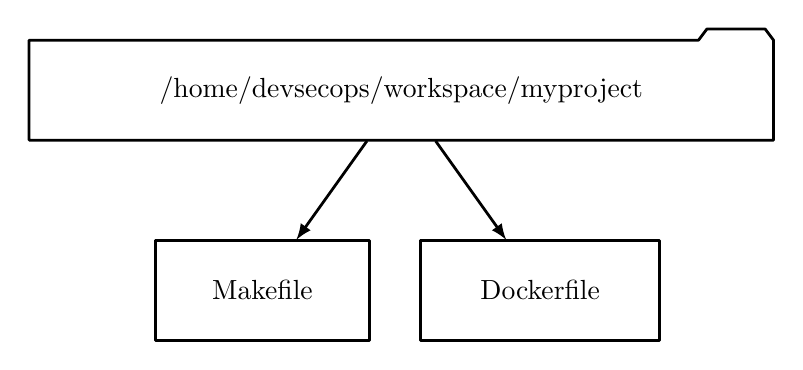
\begin{tikzpicture}[>=latex,line join=bevel,]
  \pgfsetlinewidth{1bp}
%%
\pgfsetcolor{black}
  % Edge: devsecops -> Makefile
  \draw [->] (121.64bp,71.697bp) .. controls (115.77bp,63.474bp) and (108.63bp,53.483bp)  .. (96.217bp,36.104bp);
  % Edge: devsecops -> Dockerfile
  \draw [->] (146.36bp,71.697bp) .. controls (152.23bp,63.474bp) and (159.37bp,53.483bp)  .. (171.78bp,36.104bp);
  % Node: devsecops
\begin{scope}
  \definecolor{strokecol}{rgb}{0.0,0.0,0.0};
  \pgfsetstrokecolor{strokecol}
  \draw (268.0bp,108.0bp) -- (265.0bp,112.0bp) -- (244.0bp,112.0bp) -- (241.0bp,108.0bp) -- (0.0bp,108.0bp) -- (0.0bp,72.0bp) -- (268.0bp,72.0bp) -- cycle;
  \draw (134.0bp,90.0bp) node {/home/devsecops/workspace/myproject};
\end{scope}
  % Node: Makefile
\begin{scope}
  \definecolor{strokecol}{rgb}{0.0,0.0,0.0};
  \pgfsetstrokecolor{strokecol}
  \draw (122.5bp,36.0bp) -- (45.5bp,36.0bp) -- (45.5bp,0.0bp) -- (122.5bp,0.0bp) -- cycle;
  \draw (84.0bp,18.0bp) node {Makefile};
\end{scope}
  % Node: Dockerfile
\begin{scope}
  \definecolor{strokecol}{rgb}{0.0,0.0,0.0};
  \pgfsetstrokecolor{strokecol}
  \draw (227.0bp,36.0bp) -- (141.0bp,36.0bp) -- (141.0bp,0.0bp) -- (227.0bp,0.0bp) -- cycle;
  \draw (184.0bp,18.0bp) node {Dockerfile};
\end{scope}
%
\end{tikzpicture}


	\caption{Makefile and related files.}
\label{makefile}
\end{figure}

